\documentclass[conference]{IEEEtran}
% \IEEEoverridecommandlockouts
% The preceding line is only needed to identify funding in the first footnote. If that is unneeded, please comment it out.
\usepackage{cite}
\usepackage{amsmath,amssymb,amsfonts}
\usepackage{algorithmic}
\usepackage{hyperref}
\usepackage{graphicx}
\usepackage{textcomp}
\usepackage{xcolor}
\def\BibTeX{{\rm B\kern-.05em{\sc i\kern-.025em b}\kern-.08em
    T\kern-.1667em\lower.7ex\hbox{E}\kern-.125emX}}
\begin{document}

\title{Computer Technology Project I\\}

\author{\IEEEauthorblockN{Simon Nyman}
\IEEEauthorblockA{\textit{Dept. of Electrical and Computer Engineering  (of Aff.)} \\
\textit{Aarhus University}\\
Studentnumber: 202305077\\}
\and
\IEEEauthorblockN{Jakob Palm}
\IEEEauthorblockA{\textit{Dept. of Electrical and Computer Engineering} \\
\textit{Aarhus University}\\
Studentnumber: 202307244\\}
}

\maketitle

\begin{abstract}
\end{abstract}

\section{Introduction}
The goal for this project was to design a down-scaled version of a Search And Rescue (SAR) robot, used to rescue victims in the aftermaths of natural disasters.
The robot will imitate a real world scenario by, autonomously navigating an obstacle course and distinguishing between different color markings, representing potential victims. To achieved this we use the TurtleBot3 Burger Robot equipped with different sensors.
All the software will be implmented in python using the Robot Operating Software framework (ROS). For the sensors we will be using a LiDAR sensor capable of measuring distances in a 360 degree view, and an RGB-sensor which differentiates between red, green and blue colors. 
The performance will be assesd based on three factors: Average speed, number of collisions and "victims" found.

\section{Specifications}
Our Search and Rescue implementation used a turtlebot3 robot, specifically the burger configuration with dimensions 138mm x 178mm x 192mm (L $\times$ W $\times$ H)\cite{b1}.
On the turtlebot3, a Raspberry Pi 3 model B+ and an Arduino are connected in order to process the incoming external signals from the various sensors.
Furthermore, the robot has two motors attached, one for each wheel. From the specification it is evident that the robot has a maximal linear velocity of 0.22 m/s
and a maximum rotational velocity of 2.84 rad/s. In order keep the robot as agile as possible with no wires attached, we used an 800 mA Li-Po battery and established a wireless connection, which will be specified further in a following section.
The specific RGB used is an ISL29125 low power, high sensitivity red, green and blue light sensor with SMBus compatibility\cite{b2}.
The LiDAR used is the LDS-01 version with a range of 120 mm to 3500 mm \cite{b3}

\subsection{Software Setup}

\subsubsection{Network Configuration}
As mentioned, we wanted the robot to be able to move as freely as possible, meaning that connecting it to our machine via an ethernet cable was not the way to go.
Therefore, we established a wireless connection to the robot by changing the network configuration on the pi. We used the following command:


\subsubsection{ROS}


\section{Methodology and Design}
Throughout the project we have been using the trial and error approach, which allowed for an efficent overall workflow.
This approach works well, when having to build and optimize code for hardware, as we would need to see if and how the code is working.
Furthermore, this approach works in great synergy with the See-Think-Act Cycle we use for the robot \hyperref[sec:STAC].
We are able to edit the "see", "think" and "act" parts individually and get instant feedback by testing, simplifying both the building and optimization processes.
\begin{figure}[htbp]
    \centerline{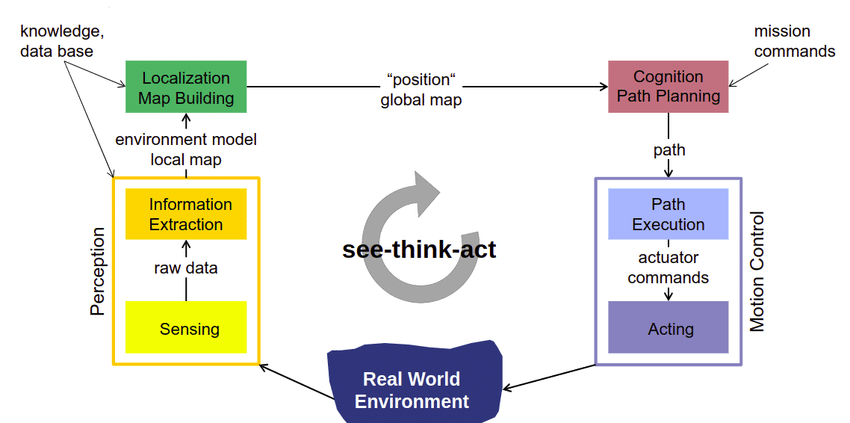
\includegraphics[width=1.0\columnwidth]{STAC.png}}
    \caption{Robots See-Think-Act Cycle.}
    \label{sec:STAC}
    \end{figure}


\subsection{Navigation}
implementation
\subsection{RGB}
implementation
\subsection{LED}
implementation
\section{Experimentation and Testing}

\section{Conclusion}

\section{Discussion}


\begin{thebibliography}{00}
\bibitem{b1} 'Turtlebot3 features', accessed 15 May 2024, available at: https://emanual.robotis.com/docs/en/platform/turtlebot3/features/
\bibitem{b2} 'Renesas RGB-sensor ISL29125 datasheet', accessed 15 May 2024, available at: https://www.alldatasheet.com/datasheet-pdf/pdf/1045936/RENESAS/ISL29125.html
\bibitem{b3} 'LDS-01 overview', accessed 15 May 2024, available at: https://www.robot-advance.com/EN/art-360-laser-distance-sensor-lds-01-2352.htm
\end{thebibliography}

\end{document}
